\documentclass[aps,onecolumn,groupedaddress,nofootinbib,pra]{revtex4-2}
\pdfoutput=1

\newcommand{\mainDocFilename}{chaotic-kummer-v1} %

\usepackage{lineno}
\usepackage{amssymb,amsmath,amsthm}
\usepackage[shortlabels]{enumitem}
\usepackage{braket}
\usepackage{comment}
\usepackage{subcaption}
\DeclareCaptionJustification{block}{\leftskip=0pt\rightskip=0pt\parfillskip=0pt plus 1fil\relax}
\captionsetup{justification=block}
\usepackage{graphicx, xcolor, varwidth}
\usepackage{color}
\usepackage{csquotes} 
\usepackage{mathtools}
\usepackage{tikz}
\usepackage{commath}
\usepackage{adjustbox}
\usepackage{booktabs}
\usepackage{placeins}
\usepackage{xr-hyper}
\usepackage{hyperref}
\usepackage{dsfont}

\hypersetup{
    pdfstartview={FitH},
    pdftitle={Onset of quantum chaos in a family of two-dimensional conformal field theories - SM},
    pdfauthor={Felix M. Haehl, Moshe Rozali},
    colorlinks=true,
    linkcolor=cyan,
    citecolor=cyan,
    filecolor=magenta,
    urlcolor=blue
}

\makeatletter
\renewcommand\paragraph{\@startsection{paragraph}{4}{\parindent}{\z@}{-1em}{\normalfont\normalsize\bfseries}}
\makeatother

\newcommand{\Sym}{\mathrm{Sym}}
\newcommand{\Tf}{\mathbb T^4}
\newcommand{\Def}{\mathcal D} 
\newcommand{\B}{\mathcal B}
\newcommand{\HB}{H_{\B}}
\newcommand{\DB}{D_{\B}}
\newcommand{\MB}{M_{\B}}
\newcommand{\cMat}{{\rm c}}
\newcommand{\twist}{{\boldsymbol\sigma}}
\newcommand{\lam}{\lambda}
\newcommand{\Lam}{\Lambda}
\newcommand{\Gt}{\widetilde G}
\newcommand{\rmean}{\langle r\rangle}
\newcommand{\bs}{\mathbf s}
\newcommand{\bt}{\mathbf t}
\newcommand{\bff}{\mathbf f}
\newcommand{\bn}{\mathbf n}
\newcommand{\ba}{\mathbf a}
\newcommand{\bb}{\mathbf b}
\newcommand{\bw}{\mathbf w}
\newcommand{\Ovol}{\mathcal O_{\rm vol}}
\newcommand{\Dc}{\Def_{\cMat}}
\newcommand{\Mc}{M_{\cMat}} 
\newcommand{\Hc}{{\cal G}_{\cMat}}
\newcommand{\Dcz}{\Def_{\cMat,0}}
\newcommand{\jj}{\mathrm j}
\newcommand{\kk}{\mathrm k}
\newcommand{\om}{\omega}
\newcommand{\PsiE}{\Psi^{_{(E)}}}
\DeclareMathOperator{\Tr}{Tr}
\DeclareMathOperator{\lcm}{lcm}
\DeclareMathOperator{\spec}{spec}
\DeclareMathOperator{\rank}{rank}

\externaldocument[M-][nocite]{\mainDocFilename}
\begin{document}
\ifdefined\arXivversion
  \begin{center}\large\bfseries Supplemental Material\end{center}
  \setcounter{section}{0}
  \setcounter{table}{0}
\else
  \title{Supplemental Material: Onset of quantum chaos in a family of two-dimensional conformal field theories}
  \author{Felix M.\ Haehl}
  \author{Moshe Rozali}
  \maketitle
\fi
\setcounter{secnumdepth}{1}
\setcounter{equation}{0}
\setcounter{figure}{0}
\renewcommand{\thesection}{S\arabic{section}}
\renewcommand{\theequation}{S\arabic{equation}}
\renewcommand{\thefigure}{S\arabic{figure}}
\renewcommand{\thetable}{S\arabic{table}}
\renewcommand{\theHsection}{S\arabic{section}}
\renewcommand{\theHequation}{S\arabic{equation}}
\renewcommand{\theHfigure}{S\arabic{figure}}
\renewcommand{\theHtable}{S\arabic{table}}



\section{The Kummer point and its symmetry sectors}
\label{app:kummer}

\paragraph*{States on the torus.}
The free fields obey the reality conditions $(X_{A\dot A})^*=-X^{A\dot A}$, $(\psi^{\alpha A})^\dagger=-\psi_{\alpha A}$ and $(\bar\psi^{\dot\alpha A})^\dagger=-\bar\psi_{\dot\alpha A}$, with all indices raised and lowered by $\epsilon_{+-}=1=-\epsilon^{+-}$, so that $\psi^{\alpha A}$ and $\bar\psi^{\dot\alpha A}$ each contain two complex fermions \cite{Avery:2010er}. The four real components of $X_{A\dot A}$ can be traded for four bosonic coordinates along the four orthogonal circles of $\Tf$, $X^i$ $(i=1,\dots,4)$, each obeying $X^i\sim X^i+2\pi R$. On a single circle the states carry an integer momentum $n$ and an integer winding $w$. In units $\alpha'=2$, in which the self-dual radius is $\sqrt2$, their momenta and weights are:
\begin{equation}
\label{eq:circle}
p_{L,R}=\frac{n}{R}\pm\frac{wR}{2}\,,\qquad h=\frac12\,p_L^2+N_L\,,\qquad \bar h=\frac12\,p_R^2+N_R\,.
\end{equation}
At the free-fermion radius $R=2$, where each compact boson is equivalent to a free Dirac fermion, the momenta $a\equiv p_L=\frac n2+w$ and $b\equiv p_R=\frac n2-w$ are half-integers with $a-b=2w$ even. Conversely, every such pair $(a,b)$ belongs to a state with $n=a+b$ and $w=\frac12(a-b)$. Repeating this construction on all four circles of $\Tf$ gives the weights
\begin{equation}
\label{eq:weights}
h=\frac12|\ba|^2+N_L\,,\qquad \bar h=\frac12|\bb|^2+N_R\,,
\end{equation}
with oscillator levels $N_{L,R}\in\mathbb Z_{\ge0}$, left- and right-moving momenta $\ba,\bb\in(\frac12\mathbb Z)^4$ subject to $\ba-\bb\in2\mathbb Z^4$, integer momentum $\bn=\ba+\bb$ and winding $\bw=\frac12(\ba-\bb)$. The spin $h-\bar h=\frac12(\ba-\bb)\cdot(\ba+\bb)+N_L-N_R=\bn\cdot\bw+N_L-N_R$ is an integer, as it must be. Figure~\ref{fig:sectors} (left) shows the momenta $(a_i,b_i)$ of one circle.\\

\begin{figure}[htb]
\centering
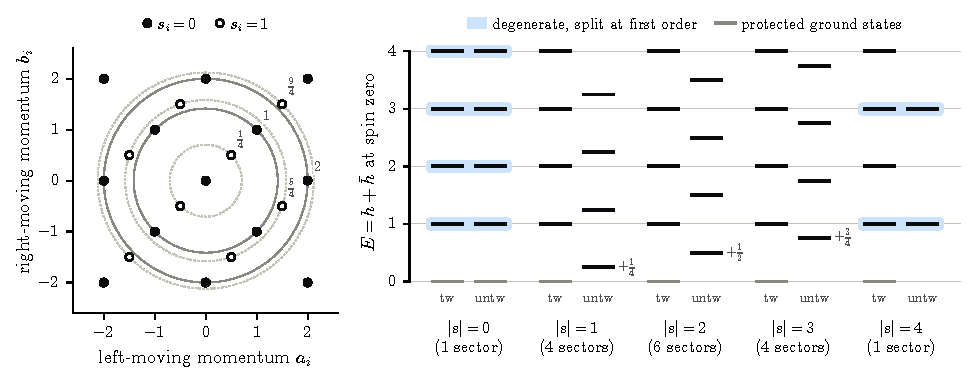
\includegraphics[width=0.85\textwidth]{fig_kummer_sectors.pdf}
\caption{The levels of the Kummer point by symmetry sector. {\it Left:} The left- and right-moving momenta $(a_i,b_i)$ of one circle of the torus: integer momenta ($s_i=0$) have integer energy $\tfrac12(a_i^2+b_i^2)$, half-integer ones ($s_i=1$) are shifted by $\tfrac14$. The circles are curves of constant energy $\tfrac12(a_i^2+b_i^2)$, labeled by its value (solid for $s_i=0$, dotted for $s_i=1$). {\it Right:} There are $16$ symmetry sectors labeled by $\bs \in \{0,1\}^4$. We show the twisted (tw) and untwisted (untw) energies of the spin-zero states in the sectors of weight $|\bs|$. The twisted tower \eqref{M-eq:weights_tw} is the same in every sector, while the untwisted energies lie on $\mathbb Z+\frac14 |\bs|$ (only on the odd integers for $|\bs|=4$). Twisted and untwisted states are degenerate only for $|\bs|=0$ and at the odd levels for $|\bs|=4$ (shaded).}
\label{fig:sectors}
\end{figure}

For each allowed momentum pair $(\ba,\bb)$, let $|\ba,\bb;0_R\rangle$ denote the Ramond oscillator vacuum of lowest left- and right-moving R-charge. We write the Fock-space states in the form:
\begin{equation}
|\ba,\bb;I_L,I_R\rangle_{\Tf} = {\cal O}_{I_L}\,\bar{\cal O}_{I_R}
|\ba,\bb;0_R\rangle\,,
\end{equation}
where $I_L,I_R$ specify the modes, polarizations and occupation numbers of the creation operators. The oscillator monomials are understood to be normalized and may include creation operators for fermion zero modes.\\

\paragraph*{The orbifold.}
The reflection maps a state of momenta $(\ba,\bb)$ to one of momenta $(-\ba,-\bb)$ and reverses the sign of every oscillator, including the fermion zero modes. The untwisted sector consists of the even combinations of a state and its image: each pair $(\ba,\bb)\neq(0,0)$ gives one reflection-invariant combination:
\begin{equation}
|\ba,\bb;I_L,I_R\rangle_{\text{untw}} \propto |\ba,\bb;I_L,I_R\rangle_{\Tf} + (-1)^{k_L+k_R} \, |-\ba,-\bb;I_L,I_R\rangle_{\Tf}\,,
\end{equation}
where $k_L$ ($k_R$) counts the creation operators in ${\cal O}_{I_L}$ ($\bar {\cal O}_{I_R}$). For $\ba=\bb=0$ the states with an even number of oscillator excitations $k_L+k_R$ survive as well. 

In the twisted sectors the fields are only periodic up to reflection, $X(\sigma+2\pi)=-X(\sigma)$. A twisted-sector string must be localized at a fixed point $x\equiv-x$ of the reflection, i.e., at one of the $16$ half-period points $x_\bff=\pi R\,\bff$, $\bff\in\{0,1\}^4$, so the twisted sector is a direct sum of $16$ fixed-point sectors (one for each conjugacy class of reflections in the space group of the torus). All its fields are antiperiodic, so their modes are half-integer and there are no momenta or windings. The zero-point energy of each of the four antiperiodic bosons lies $\frac1{16}$ higher than that of a periodic boson. Similarly, each of the four antiperiodic fermions lies $\frac1{16}$ below that of a Ramond fermion. The two cancel, so the ground state of every twisted sector has $h=\bar h=0$, exactly like the Ramond ground state of the untwisted sector. Every twisted mode is odd under the reflection and the twisted ground state is even, so a state built with $k$ modes has parity $(-1)^k$, while its total level $N^{\rm tw}_L+N^{\rm tw}_R$ lies in $\frac{1}{2}k+\mathbb Z$. The projection onto even states gives \eqref{M-eq:weights_tw}, and the tower is the same at every fixed point.\\

\paragraph*{Symmetry sectors.}
To organize the twisted states by the same quantum numbers as the untwisted states, we pass from the basis labeled by fixed points to the simultaneous eigenbasis of the half-period translations. The half-period translations $U_\bt\colon x \mapsto x+\pi R\, \bt$ commute with the orbifolding reflection, since $-(x+\pi R\,\bt)\equiv-x+\pi R\,\bt$ up to a lattice vector. The translations form a symmetry group $\mathbb Z_2^4$. We label its simultaneous eigenspaces by $\bs\in\{0,1\}^4$, specifying their joint eigenvalues:
\begin{equation}
 {\cal H}_\bs = \left\{ |\Psi\rangle: \quad U_\bt |\Psi\rangle = (-1)^{\bs \cdot \bt} |\Psi \rangle \text{ for every } \bt \right\} \,.
\end{equation} 
These symmetry sectors are not to be confused with the twisted and untwisted sectors, since each contains states of both kinds. On an untwisted state, $U_\bt$ acts by the phase $(-1)^{\bn\cdot\bt}$, so its symmetry label is $\bs=\bn\bmod2=(2\ba)\bmod2=(2\bb)\bmod2$. This means that in the sector $\bs$, the momenta $a_i$ and $b_i$ are integers for $s_i=0$ and half-integers for $s_i=1$. The twisted sectors are associated with the fixed points $x_{\bff} = \pi R \, \bff$ and thus they are permuted by the translations, $U_{\bt} \colon x_{\bff} \mapsto x_{\bff + \bt}$. The action of $U_\bt$ is diagonalized by the following combinations:
\begin{equation}
\label{eq:twcomb}
|\bs\rangle_{\rm tw}=\frac14\sum_{\bff\in\{0,1\}^4}(-1)^{\bs\cdot\bff}\,|\bff\rangle 
\qquad \Rightarrow \qquad U_\bt   |\bs\rangle_{\rm tw} = (-1)^{\bs\cdot\bt}\,|\bs\rangle_{\rm tw} \,,
\end{equation}
where $|\bff\rangle$ denotes the normalized twisted Ramond ground state at $x_\bff$. Since translations leave the oscillator modes unchanged, the same Fourier combinations organize every oscillator excitation into the corresponding symmetry sector. Each sector $\bs$ therefore contains the untwisted states with momentum $\bn\equiv\bs\bmod2$ and one copy of the twisted tower built on $|\bs\rangle_{\rm tw}$. The invariant sector $\bs=0$ contains the untwisted states of even momentum and the symmetric combination of the fixed-point sectors.

Permutations of the four circles are symmetries of the square torus, so two sectors whose labels differ by a permutation are isospectral. The $15$ sectors with $\bs\neq 0$ fall into four classes, labeled by the weight $|\bs|=1,2,3,4$ (the number of non-zero components of $\bs$), with $4$, $6$, $4$ and $1$ members. On a circle with $s_i=0$ the energy $\frac12(a_i^2+b_i^2)$ is an integer, while on a circle with $s_i=1$ it is an integer plus $\frac14$ (see Fig.~\ref{fig:sectors}). The untwisted energies of a sector $\bs$ therefore lie on $\mathbb Z+\frac14|\bs|$, whereas the twisted energies are integers in every sector. Twisted and untwisted states can thus be degenerate only in the invariant sector and in the sector of weight four. Since our marginal deformations only connect untwisted to twisted states, at first order they act only within blocks that contain states of both kinds. In the $14$ sectors of weight $|\bs|=1,2,3$ there are no such blocks: the first-order shifts vanish, and the degeneracies are lifted only at second order. In the sector of weight $|\bs|=4$ all momenta are half-integers, so $|\ba|^2$ is odd, and the energies $E=|\ba|^2+2N_L$ of its spin-zero untwisted states are odd integers. That sector therefore mixes twisted and untwisted states at first order only at its odd levels.\\

\paragraph*{The involution $Z_R$.}
The reversal of the right-moving fields alone, $(\bar\partial X,\bar\psi)\to-(\bar\partial X,\bar\psi)$, maps the momenta $(\ba,\bb)$ to $(\ba,-\bb)$:
\begin{equation}
 Z_R |\ba,\bb;I_L,I_R\rangle_{\text{untw}} = (-1)^{k_R} \, |\ba,-\bb;I_L,I_R \rangle_{\text{untw}} \,.
\end{equation}
This respects $\ba-\bb\in2\mathbb Z^4$ only if $\ba+\bb\in2\mathbb Z^4$, i.e., in the invariant sector $\bs=0$. Thus, $Z_R$ acts only in this sector. It commutes with the reflection, with the point group and with both $\mathcal N=4$ algebras, whose right-moving generators are even, so it maps the space of states to itself. On the oscillator vacua, we choose the conventional sign $Z_R |\ba,\bb;0_R\rangle = +|\ba,-\bb;0_R\rangle$.

First, consider the action of $Z_R$ on the twisted states. It reverses every right-moving mode, so with $Z_R=+1$ on the twisted ground state, a twisted state with $k_R$ right-moving modes has $\bar h\in\frac{1}{2}k_R+\mathbb Z$ and $Z_R=(-1)^{k_R}=(-1)^{2\bar h}$, which evaluates to $Z_R=(-1)^E$ for a scalar of level $E$.

Next, consider untwisted states. At an odd level, both $|\ba|^2=E-2N_L$ and $|\bb|^2=E-2N_R$ are odd, so neither $\ba$ nor $\bb$ vanishes. The momentum pairs $\{\pm(\ba,\bb)\}$ and $\{\pm(\ba,-\bb)\}$ are therefore disjoint and $Z_R$ maps the first pair to the second and vice versa. Its two eigenspaces at that level thus have equal dimensions. In particular, the number of untwisted primaries with $Z_R=(-1)^E$, which can couple to the twisted states, is $\tilde d_+=\frac12 d_+$.

Finally, we note that the marginal deformations preserve $Z_R$: indeed, as one can check explicitly for any oscillator excitation using the covering-space construction, the right-moving twist maps satisfy:
\begin{equation}
 \langle Z_R t_R|{\cal A}_{\dot B}|Z_R u_R\rangle
 =\langle t_R|{\cal A}_{\dot B}|u_R\rangle \,.
\end{equation}
Since the $\Dc$ matrix elements chirally factorize and $Z_R$ only acts on the right-moving half, it follows that $[Z_R,\Dc]=0$ on the invariant sector ${\cal H}_{\bs = 0}$.\\

\paragraph*{States used in the calculation.}
With the restriction to spin-zero Ramond states understood (Sec.~\ref{M-sec:theory}), we retain one primary from each copy of an irreducible massive representation of the two $\mathcal N=4$ algebras at $E>0$. In each chirality, its lowest-energy subspace contains an R-spin-$\frac12$ doublet and two singlets. We choose the lowest-weight component $|P\rangle$, characterized by:
\begin{equation}
\begin{split}
J^3_0|P\rangle &=-\tfrac12|P\rangle\,,\qquad G^-_{\dot A,0}|P\rangle=0\,,\\
L_n|P\rangle &=J^a_n|P\rangle =G^\alpha_{\dot A,n}|P\rangle=0 \qquad(n\geq1)\,,
\end{split}
\end{equation}
and similarly with bars. Applying these conditions to the orbifold Fock spaces, we construct complete orthonormal bases of $\B(E)$ for $0<E\le8$.

At $E=0$, our R-charge conditions select only the protected Ramond vacuum (Sec.~\ref{M-sec:theory}). For each level $E\leq 8$, we diagonalize the first-order deformation on the space of these primaries. States at other energies do not enter its first-order splitting.


\section{The marginal deformations}
\label{app:deformations}

\paragraph*{Supercurrents.}
In each chirality the free theory has a small $\mathcal N=4$ superconformal symmetry with $c=6$. In the conventions of \cite{Avery:2010er} the left-moving generators are the stress tensor, the $SU(2)_L$ R-currents and four supercurrents:
\begin{equation}
\label{eq:N4gen}
T=-\frac12(\partial X^\dagger)^{A\dot A}\partial X_{A\dot A}-\frac12(\psi^\dagger)_{\alpha A}\partial\psi^{\alpha A}\,,\qquad
J^a=-\frac14(\psi^\dagger)_{\alpha A}(\sigma^{Ta})^{\alpha}{}_{\beta}\,\psi^{\beta A}\,,\qquad
G^\alpha_{\dot A}=\psi^{\alpha A}\partial X_{A\dot A}\,,
\end{equation}
where $\sigma^a$ are the Pauli matrices. The right-moving generators are built in the same way from the right-moving fermions and the right-moving current of the same bosons. The supercurrents have $h=\frac32$. They are doublets of $SU(2)_L$, so that $G^{\pm}$ raise and lower the R-charge by $\frac12$, doublets of $SU(2)_2$, and singlets of $SU(2)_1$. Their modes obey $(G^\alpha_{\dot A,r})^\dagger=\epsilon_{\alpha\beta}\,\epsilon^{\dot A\dot B}\,G^{\beta}_{\dot B,-r}$, so they amount to two complex supercurrents \cite{Guo:2019ady}. The modes $G^\alpha_{\dot A,r}=\oint\frac{dz}{2\pi i }\,z^{r+\frac12}\,G^\alpha_{\dot A}(z)$ satisfy \cite{Avery:2010er}:
\begin{equation}
\label{eq:GG}
\{G^\alpha_{\dot A,m},G^\beta_{\dot B,n}\}=\epsilon_{\dot A\dot B}\left[\left(n^2-\frac14\right)\epsilon^{\alpha\beta}\delta_{m+n,0}
+(m-n)(\sigma^{aT})^{\alpha}{}_{\gamma}\,\epsilon^{\gamma\beta}J^a_{m+n}+\epsilon^{\alpha\beta}L_{m+n}\right]\,,
\end{equation}
where, as usual, $r\in \mathbb{Z}$ in the Ramond sector, while $r\in \frac12+\mathbb{Z}$ in the NS sector. A chiral primary is a superconformal primary that is annihilated by $G^{+}_{\dot A,-\frac12}$, and its weight equals its R-spin, $h=j$. Acting on a chiral primary with $h=j=\frac12$ on both sides, $G^{-}_{\dot A,-\frac12}\bar G^{-}_{\dot B,-\frac12}$ gives an R-singlet of weights $(1,1)$, the top component of a short multiplet. Integrated over the worldsheet, such an operator is an exactly marginal deformation that preserves $\mathcal N=(4,4)$ supersymmetry.\\

\paragraph*{The singlet and triplet deformations.}
In the D1-D5 literature the undeformed theory is the symmetric orbifold $\Sym^N(\Tf)$, and the deformation is built on the twist field $\twist^{\beta\dot\beta}$ of the sector in which two copies of the torus theory are exchanged \cite{Avery:2010er,Guo:2019ady}. It is a doublet of $SU(2)_L\times SU(2)_R$ with $h=\bar h=j=\bar j=\frac12$, whose highest R-weight component $\twist^{++}$ is a chiral primary \cite{Avery:2010er}. The standard deformation operator takes the form \cite{Guo:2019ady}:
\begin{equation}
\label{eq:Dstandard}
D=\frac14\,\epsilon^{\dot A\dot B}\epsilon_{\alpha\beta}\epsilon_{\dot\alpha\dot\beta}\,G^{\alpha}_{\dot A,-\frac12}\,
\bar G^{\dot\alpha}_{\dot B,-\frac12}\,\twist^{\beta\dot\beta}
=\epsilon^{\dot A\dot B}\,G^{-}_{\dot A,-\frac12}\,\bar G^{-}_{\dot B,-\frac12}\,\twist^{++}\,,
\end{equation}
where in the second step we used $G^{+}_{\dot A,-\frac12}\twist^{-\dot\beta}=-G^{-}_{\dot A,-\frac12}\twist^{+\dot\beta}$, so that $\epsilon_{\alpha\beta}G^\alpha_{\dot A,-\frac12}\twist^{\beta\dot\beta}=-2\,G^{-}_{\dot A,-\frac12}\twist^{+\dot\beta}$, and similarly for the right-movers. The contraction of the indices makes $D$ an R-singlet of weights $(1,1)$, and the contraction of the $SU(2)_2$ indices with $\epsilon^{\dot A\dot B}$ makes it invariant under the rotations of the torus. With $\epsilon^{+-}=-1$ the coefficient matrix $\epsilon^{\dot A\dot B}$ is $- i \sigma_y$, which is the direction we call the singlet. Replacing it by one of the symmetric matrices $1$, $ i \sigma_x$ and $ i \sigma_z$ gives the three components of an $SU(2)_2$ triplet of deformations, which preserves supersymmetry and R-symmetry without being invariant under $SU(2)_2$ \cite{Gaberdiel:2025smz}. The Kummer model has the same structure, with the reflection twist fields at its $16$ fixed points in place of the twist field that exchanges two copies, and we allow the $SU(2)_2$ indices to be contracted with an arbitrary coefficient matrix.\\

\paragraph*{Hermiticity and normalization.}
The general $\mathbb Z_2^4$-symmetric deformation with a complex coefficient matrix $\cMat^{\dot A\dot B}$ is made Hermitian by adding its conjugate:
\begin{equation}
\label{eq:Dherm}
\Dc
 =\frac{1}{2\sqrt{2}} \left[ \cMat^{\dot A\dot B}\,G^{-}_{\dot A,-\frac12}\,\bar G^{-}_{\dot B,-\frac12}\,\twist^{++}  + \cMat^*_{\dot A\dot B}  \;\epsilon^{\dot A\dot C}G^{+}_{\dot C,-\frac12}\;\epsilon^{\dot B\dot D}\bar G^{+}_{\dot D,-\frac12} \;\twist^{--} \right]
 =\frac{1}{2\sqrt{2}} \,(\cMat+\epsilon \cMat^*\epsilon^T)^{\dot A \dot B}\,G^{-}_{\dot A,-\frac12}\,\bar G^{-}_{\dot B,-\frac12}\,\twist^{++}\,,
\end{equation}
where $\cMat^*_{\dot A\dot B} \equiv (\cMat^{\dot A \dot B})^*$ (indices lowered by complex conjugation). This depends only on the matrix $\mathfrak{c} = \frac12(\cMat+\epsilon \cMat^*\epsilon^T)$, which satisfies $\mathfrak{c} ^*=\epsilon\, \mathfrak{c} \,\epsilon^T$. Without loss of generality $\cMat$ is therefore a real quaternion, \eqref{M-eq:quaternion}, and $\Dc$ takes the form \eqref{M-eq:Dc}. An overall phase $\cMat\to e^{ i \theta}\cMat$ would only rescale $\Dc$ by $\cos\theta$, which can be absorbed into $\lam$. The four operators $G^{-}_{\dot A,-\frac12}\bar G^{-}_{\dot B,-\frac12}\twist^{++}$ are orthonormal, since $\twist^{++}$ has unit norm and, by \eqref{eq:GG}, the states $G^{-}_{\dot A,-\frac12}|\twist^{+}\rangle$ have unit norm and are orthogonal for the two values of $\dot A$. Hence the two-point function takes the form:
\begin{equation}
\label{eq:norm}
\langle\Dc(z)\Dc(0)\rangle=\frac{\Tr (\cMat \cMat^\dagger)}{2|z|^{4}}=\frac{|q|^2}{|z|^{4}}\,,
\end{equation}
and we choose $|q|=1$. Every $\Dc$ is exactly marginal, and the deformed theory is the K3 sigma model at a neighboring point of its moduli space, with $c=6$ unchanged \cite{Seiberg:1999xz}.


\section{Symmetries of a direction}
\label{app:symmetries}

\paragraph*{Continuous symmetries.}
The currents $i\partial X$ and $i\bar\partial X$ of the torus, whose charges are the momenta $\ba$ and $\bb$, are odd under the reflection, so the orbifold has already projected them out. In the orbifold the momenta label the untwisted states only up to a common sign and the twisted states do not carry momenta. Among the translations only the half-period shifts $\mathbb Z_2^4$ survive (cf.\ Sec.~\ref{app:kummer}). The weight-one currents of the orbifold are the fermion bilinears, which generate an $su(2)\oplus su(2)$ current algebra at level one in each chirality \cite{Nahm:1999ps,Gaberdiel:2025smz}. On the left-movers, one factor rotates the index $\alpha$ and commutes with the R-singlet $\Dc$. The other factor rotates the index $A$ of the fermions but not that of the bosons, so it does not commute with the supercurrents $G^\alpha_{\dot A}=\psi^{\alpha A}\partial X_{A\dot A}$ and is broken by $\Dc$. Only the two copies of the $\mathcal N=4$ algebra remain as continuous symmetries. These are resolved by working with superconformal primaries of the Ramond sector (Sec.~\ref{app:kummer}).\\

\paragraph*{Mirrors and chambers.}
The equivalences of the full theory described in End Matter act by signed permutations of $(q_0,q_1,q_3)$ and an independent reversal of $q_2$, giving $2^3\,3!\times2=96$ elements. The additional right-moving equivalences of the invariant sector (see below) enlarge this set to all signed permutations of four coordinates, with $2^4\,4!=384$ elements. This is known as the Weyl group $W(B_4)$. Away from the mirrors, the four signs and the ordering of the absolute values specify $384$ ``chambers'' on $S^3$. For example, $q_0\geq q_1\geq q_2\geq q_3\geq0$ defines a fundamental chamber whose four reflecting faces cut out a spherical tetrahedron on $S^3$. Figure~\ref{fig:mirrorgeometry} illustrates the analogous construction on $S^2$, where $2^3\,3!=48$ signed orderings give spherical triangles.\\

\begin{figure}[htb]
\centering
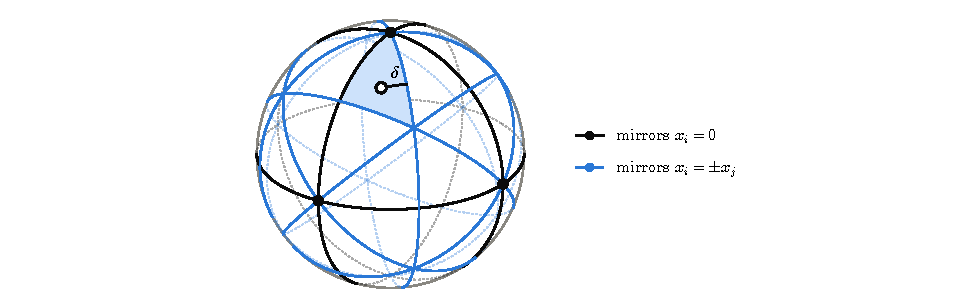
\includegraphics[width=0.8\textwidth]{fig_walls_geometry.pdf}
\caption{Mirrors $x_i=0$ and $x_i=\pm x_{j\neq i}$ on the two-sphere $S^2$. The nine mirrors are great circles, which cut the sphere into $48$ spherical triangles (the chambers of the Weyl group $W(B_3)$). The white dot is a ``generic direction'', at the angle $\delta$ from the nearest mirror.}
\label{fig:mirrorgeometry}
\end{figure}

The singlet deformation \eqref{eq:Dstandard} is the quaternion unit $q=(0,0,-1,0)$, where nine mirrors meet ($q_0=q_1=q_3=0$ and $q_\mu=\pm q_\nu$ for $\mu,\nu\in\{0,1,3\}$). The triplet deformation \cite{Gaberdiel:2025smz} is spanned by the other three quaternion units $(1,0,0,0)$, $(0,1,0,0)$ and $(0,0,0,1)$, i.e., by the mirror $q_2=0$.\\

\paragraph*{The point group and generic directions.}
The square torus $\Tf$ is symmetric under the rotations and reflections of $\mathbb R^4$ that map the lattice $\mathbb Z^4$ to itself. These are $384$ signed permutations of the coordinates, and we consider the orientation-preserving ones. We parametrize the latter as $192$ signed permutation matrices of determinant one. Since the fermions transform as spinors, we then lift the permutations to the double cover $\mathrm{Spin}(4)=SU(2)_1\times SU(2)_2$, obtaining a group $\Gt$ of order $384$. An element $(g_1,g_2)$ acts on quaternion coordinates as $x\mapsto g_1xg_2^{-1}$: $g_1$ rotates the index $A$, and $g_2$ the index $\dot A$. The four central elements $(\pm1,\pm1)$ act trivially on our chosen scalar primaries (by the orbifold projection $(-1,1)$ and even fermion parity $(-1,-1)$).

Only $g_2$ acts on the deformation coefficients. Writing its doublet matrix as $Y$, this action is $\cMat\mapsto Y\cMat Y^T$. It leaves the singlet coordinate $q_2$ unchanged and rotates the triplet $(q_0,q_1,q_3)$ by the $24$ rotations of a cube.

To a given deformation direction $\cMat$ we associate a stabilizer $\Hc$ of point-group operations that preserve the deformation. Operations sending $\cMat \mapsto -\cMat$ also qualify when combined with $\mathcal Q$ (which reverses the sign again). For a generic direction, this requires $g_2=\pm1$ and $g_1\in Q_8 =\{\pm\mathds{1},\pm i\sigma_x,\pm i\sigma_y,\pm i\sigma_z\}$. Thus $\Hc$ has $16$ elements. After quotienting by the four trivial central elements, it acts as $\mathbb Z_2\times\mathbb Z_2$, giving the four real one-dimensional characters used in the main text. Special directions can have larger stabilizers (for example, the singlet preserves all of $\Gt$).

Additional symmetries can involve worldsheet parity, which exchanges the chiralities and sends $\cMat\mapsto\cMat^T$, reversing $q_2$. It is therefore a symmetry on the mirror $q_2=0$. Its compositions with point-group operations and with ${\cal Q}$ give the symmetries on the other nine mirrors that exist in the full theory.

The six additional mirrors $q_2=\pm q_\mu$ arise from rotations of the right-moving fields alone by $(u,u)$, with $u\in\{i\sigma_x,i\sigma_y,i\sigma_z\}$. These send $\bb\mapsto u\bb u^{-1}$, changing coordinate signs and therefore preserving $\ba\equiv\bb\pmod2$ in the invariant sector. They commute with $H_0$ and preserve both $\mathcal N=4$ algebras, rotating the right-moving supercurrents among themselves. Covariance of the right-moving chiral twist maps gives $\Dcz\mapsto\mathcal D_{\cMat u,0}$ on the entire invariant sector, including matrix elements between different levels. The spectra along $\cMat$ and $\cMat u$ therefore coincide beyond first order.

Composing these rotations with the equivalences of the full theory produces the reflections in the six additional mirrors. These rotations do not preserve the full momentum-winding lattice, so the additional equivalences do not extend to the full theory. Preserving the integer lattice and its parity pairing for every allowed momentum pair restricts these right-moving rotations to $u\in Q_8$.

One further ``hidden'' $\mathbb Z_2$ of the even levels, the same along every direction, is described in End Matter; we give its explicit form at $E=2$ below.\\

\paragraph*{The hidden $\mathbb Z_2$ at $E=2$.}
The hidden $\mathbb Z_2$ (End Matter) does not depend on the direction: an involution $S$ can be found, which commutes with $H_0$, with $\Dcz$ for every $\cMat$, and with every element of $\Gt$. Along the singlet it therefore acts within each sector of $\Gt$, and it can be written down explicitly at the lowest level. At $E=2$, the sector that transforms trivially under $\Gt$ and has $Z_R=+1$ contains one twisted state and three untwisted states: the invariant oscillator state $|{\rm osc}\rangle$ ($\ba=\bb=0$); the combination $|{\rm m}{+}{\rm w}\rangle=\frac1{\sqrt2}\big(|{\rm m}\rangle+|{\rm w}\rangle\big)$ of the invariant pure-momentum state $|{\rm m}\rangle$ ($\bb=\ba$, $|\ba|^2=2$) and pure-winding state $|{\rm w}\rangle$ ($\bb=-\ba$), which are exchanged by $Z_R$; and the invariant state $|{\rm mw}\rangle$ with $|\ba|^2=|\bb|^2=2$, $\bb\neq\pm\ba$. For suitable phases of these normalized states, $S$ acts on them as the reflection
\begin{equation}\label{eq:Sreflection}
S=\frac{2\,|v\rangle\langle v|}{\langle v|v\rangle}-1\,,\qquad |v\rangle=2\,|{\rm osc}\rangle+|{\rm m}{+}{\rm w}\rangle-|{\rm mw}\rangle\,,
\end{equation}
and as $-1$ on the twisted state (the overall sign of $S$ is a convention). Along the singlet, $|v\rangle$ therefore stays at $E=2$ to first order. Note that $S$ mixes an oscillator state with momentum states of the same energy, which no automorphism of the momentum lattice can do; it is therefore not in the point group, and it is not $Z_R$, worldsheet parity or $\mathcal Q$.\\

\paragraph*{The antiunitary symmetry and symmetry class.}
Since $\Dc$ is a Hermitian scalar, CPT maps $\Dc(\sigma,0)$ to $\Dc(-\sigma,0)$ and therefore commutes with its spatial integral $\Dcz$. Composing CPT with the Weyl reflections of both R-symmetry groups returns the R-charges to our chosen lowest weights and defines an antiunitary operator $T$. The Weyl reflections preserve the R-singlet deformation, so
\begin{equation}
T H_0 T^{-1}=H_0\,,\qquad
T\Dcz T^{-1}=\Dcz \,.
\end{equation}
In the free field realization, $T$ conjugates the coefficients of Fock monomials, acts by $i\sigma_y$ on each internal index $A$ and $\dot A$, and it reverses the momenta, leaving the R-symmetry indices unchanged. Since $(i\sigma_y)^2=-1$, its square is $+1$ on bosonic oscillators, which carry both internal indices, and $-1$ on fermionic oscillators, which carry only $A$. The chosen untwisted Ramond vacuum and the twisted ground states are preserved up to phases, so $T^2=+1$ on these states. Therefore,
\begin{equation}
T^2=(-1)^F=+1
\end{equation}
on our selected space: the fixed left- and right-moving R-charges require even total fermion parity in both sectors.

The operator $T$ commutes with $\Hc$, $Z_R$ and $\mathcal Q$. For a generic direction, the characters of $\Hc$ are real, so $T$ preserves each character space and each $Z_R$ eigenspace. Where the hidden $\mathbb Z_2$ is resolved numerically (End Matter), the two jointly invariant subspaces have unequal dimensions. An antiunitary symmetry commuting with both $H_0$ and $\Dcz$ can only permute their irreducible components. Since the two components have unequal dimensions, $T$ must preserve each separately.

Since $T^2=+1$, we can choose an orthonormal basis in which $T$ acts by complex conjugation. Each fully resolved first-order matrix along a generic direction is then real symmetric. Moreover, $[T,\mathcal Q]=0$ and $\{\mathcal Q,\HB^{(1)}\}=0$ imply that the antiunitary operator $C=\mathcal Q T$ satisfies
\begin{equation}
\label{eq:Csquared}
C^2=+1\,,\qquad C\HB^{(1)}C^{-1}=-\HB^{(1)}\,.
\end{equation}
Together, these symmetries place the first-order splitting matrices $\HB^{(1)}$ in class BDI, the chiral GOE \cite{Verbaarschot:1994qf,Altland:1997zz}. Agreement of their non-zero bulk spectra with GOE statistics is tested numerically in Sec.~\ref{M-sec:firstorder}.



\section{First-order matrix and spectral statistics}
\label{app:firstorder}

\paragraph*{Relation to the symmetric orbifold.}
The twist-field construction is inherited from $\Sym^2(\Tf)$, the smallest non-trivial member of the D1-D5 symmetric orbifold family \cite{Larsen:1999uk,David:2002wn,Lunin:2001pw,Keller:2011xi,Hartman:2014oaa}. For concreteness, introduce the canonically normalized fields
\begin{equation}
X_{\rm cm}=\frac{1}{\sqrt{2}} \left(X^{(1)}+X^{(2)}\right)\,, \qquad
X_{\rm rel}=\frac{1}{\sqrt{2}} \left(X^{(1)}-X^{(2)}\right)\,.
\end{equation}
Exchange of copies preserves $X_{\rm cm}$ and reflects $X_{\rm rel}$, although their compactification lattice correlates the two. In the untwisted sector with vanishing center-of-mass momentum and winding, write $\bn_1=-\bn_2\equiv\bn$ and $\bw_1=-\bw_2\equiv\bw$.
For copies at $R_{\rm copy}=\sqrt2$ (in units $\alpha'=2$) the relative momenta are
\begin{equation}
\ba=\sqrt2\,\mathbf p_L^{(1)}=\bn+\bw\,, \qquad
\bb=\sqrt2\,\mathbf p_R^{(1)}=\bn-\bw \,.
\end{equation}
This is the invariant lattice of the radius-$2$ Kummer model, with $\bn_{\rm K}=2\bn$ and $\bw_{\rm K}=\bw$. For each choice of a center-of-mass Ramond ground state, the relative states form one copy of the invariant Kummer sector ${\cal H}_{\bs=0}$, including its twisted tower. Related twist deformation calculations through second order include
\cite{Gava:2002xb,Avery:2010er,Gaberdiel:2015uca,Keller:2019yrr,Keller:2019suk,Guo:2019ady,Guo:2020gxm}.\\

\paragraph*{Matrix elements.}
Since $\Dcz$ conserves the spin, the $\sigma$-integral in its definition gives:
\begin{equation}
\label{eq:psiprimeDpsi}
\langle\Psi_b|\Dcz|\Psi_a\rangle= \left\{ \begin{aligned} & 2\pi\,\langle\Psi_b|\Dc(0,0)|\Psi_a\rangle && \text{if } h_{\Psi_a}-\bar{h}_{\Psi_a} = h_{\Psi_b}-\bar{h}_{\Psi_b}\,, \\
&0 && \text{otherwise}\,.
\end{aligned} \right.
\end{equation}
Between two spin-zero states of the same level all four weights equal $\frac E2$. Off the level diagonal $\Dcz$ changes $E$, which matters only beyond first order. The chiral twist map ${\cal A}_{\dot A}$ sends an untwisted chiral state to the twisted chiral state produced by $G^{-}_{\dot A,-\frac12}\twist^{+}$, with $\twist^{+}$ the left-moving factor of $\twist^{++}$. A $\mathbb Z_2$ twist field reflects the fields along a loop around its insertion. On the double cover of the worldsheet branched at that point the reflected field is single-valued \cite{Dixon:1986qv}, so that a twisted-sector matrix element becomes a free-field computation on the cover. In the form of this construction developed for the symmetric orbifold \cite{Lunin:2001pw,Avery:2010er,Guo:2019ady}, the two sheets of the cover are the two copies of $\Tf$ in $\Sym^2(\Tf)$, and the reflection twist field of the Kummer torus is their exchange.

The level-preserving part of ${\cal A}_{\dot A}$ commutes with every mode of the chiral $\mathcal N=4$ algebra, zero modes included, and therefore maps massive superconformal primaries into primaries and each descendant into the corresponding descendant. The level-preserving mode of ${\cal X}=G^-_{\dot A,-\frac12}\twist^+$ is ${\cal X}_0$ (labeled by how much it lowers $L_0$). The operator product of ${\cal X}$ with any $\mathcal N=4$ generator $W$ is a total derivative, $W(w){\cal X}(z)\sim\partial_z[\Phi_W(z)/(w-z)]$, so that $[W_n,{\cal X}_k]=-k\,\Phi_{W,n+k}$, which vanishes for $k=0$. Here $\Phi_T={\cal X}$ since ${\cal X}$ is a primary of weight one, $\Phi_{J^a}=0$ since ${\cal X}$ is an R-singlet primary, and $\Phi_{G^\pm_{\dot B}}\propto\epsilon_{\dot B\dot A}\twist^\pm$ by \eqref{eq:GG}, since $\twist^+$ is a chiral primary and ${\cal X}$ an R-singlet.

To measure the statistics at a level $E$, we build $\Mc$ on the complete space of massive primaries at that level and project it onto the multiplicity spaces of the physical irreducible representations of $\Hc$. We split each of them by $Z_R$ and, at the even levels, by the hidden $\mathbb Z_2$ (End Matter). Along the singlet, $\cMat^T=-\cMat$, so worldsheet parity combined with $\mathcal Q$ is a further symmetry (Sec.~\ref{app:symmetries}), which also leads to a further splitting. In each fully resolved sub-block we retain the distinct non-zero singular values. Working in multiplicity spaces removes degeneracies due to the symmetry representations, and we additionally count any remaining exactly degenerate value only once. In our data, such additional degeneracies occur only along the singlet (Sec.~\ref{M-sec:firstorder}). We use the same distinct values for the gap ratios and for the spacing statistics. Keeping the singlet's degenerate values with their multiplicity instead makes $9\%$ of its unfolded spacings at $E=8$ exactly zero and lets the few large multiplets dominate $\Sigma^2(L)$.\\

\paragraph*{Unfolding.}
In a fully resolved sub-block, let $\nu_i$ be the distinct ordered singular values and $N(\nu)$ the number of them not larger than $\nu$ (the counting function). The smooth part $\bar N(\nu)$ of this staircase captures the mean density, which is not universal and changes from one sub-block to another, while RMT predicts the fluctuations around it. Unfolding replaces the singular values by the unfolded levels:
\begin{equation}
\label{eq:unfold}
x_i=\bar N(\nu_i)\,,\qquad i=1,\dots,n\,,
\end{equation}
which have unit mean density everywhere. In practice, we take $\bar N$ to be the least-squares fit of $N(\nu_i)=i$ by a Chebyshev polynomial in $\nu$, and we drop $5\%$ of the values at each end of the band, where the fit is least reliable. The degree of the polynomial grows with the size of the sub-block: for $n$ levels it is $n/100$ rounded to the nearest integer, and at least $12$. With one fit parameter per $100$ levels, $\bar N$ follows the mean density on scales much longer than the intervals $L\le10$ considered below. A polynomial of fixed low degree is not enough at the higher levels: at degree $12$ the fit of the larger sub-blocks leaves a residual that varies slowly across the band, which raises the number variance at large $L$. As a control, we unfolded chiral GOE spectra with the shapes of the reference direction's sub-blocks in the same way. They reproduce the GOE number variance for $L\le10$ at $E=6,7,8$, so the fit does not absorb the fluctuations on these scales. At $E=6$ the sub-blocks have between $451$ and $1366$ levels, and the fit cannot be refined further without absorbing them. Sub-blocks are unfolded separately, since their levels are uncorrelated. A sub-block is used only if the fitted staircase is monotone over the retained range, since otherwise unfolded spacings can become negative. Along the singlet direction, whose level density has sharp peaks, too few sub-blocks achieve this for $E\leq 6$, so Fig.~\ref{M-fig:spacings} shows its unfolded statistics only for $E\geq7$.\\

\paragraph*{Spacing distribution and number variance.}
The unfolded nearest-neighbor spacings $s_i=x_{i+1}-x_i$ have the distribution $P(s)$. Unlike the gap ratio, it depends on the unfolding. The Wigner surmises for the Gaussian ensembles and the distribution for uncorrelated levels read \cite{Mehta2004}:
\begin{equation}
\label{eq:wigner}
P_{\rm GOE}(s)=\frac{\pi s}{2}\,e^{-\pi s^2/4}\,,\qquad
P_{\rm GUE}(s)=\frac{32\,s^2}{\pi^2}\,e^{-4s^2/\pi}\,,\qquad
P_{\rm Poisson}(s)=e^{-s}\,.
\end{equation}
Let $n(x,L)$ be the number of unfolded levels in the interval $[x,x+L]$. Its mean is $L$ and its variance over the position of the interval,
\begin{equation}
\label{eq:sigma2}
\Sigma^2(L)=\left\langle n(x,L)^2\right\rangle_x-\left\langle n(x,L)\right\rangle_x^2\,,
\end{equation}
measures how rigid the spectrum is over $L$ levels. The universal predictions are \cite{Mehta2004}:
\begin{equation}
\label{eq:sigma2goe}
\begin{aligned}
\Sigma^2_{\rm GUE}(L)&=\frac{1}{\pi^2}\Big[\log(2\pi L)+\gamma+1-\cos(2\pi L)-\mathrm{Ci}(2\pi L)\Big]
+L\Big(1-\frac{2}{\pi}\,\mathrm{Si}(2\pi L)\Big) \, \stackrel{L\gg 1}{\approx}\, \frac{1}{\pi^2} \,\log(L) + 0.346 \,,\\
\Sigma^2_{\rm GOE}(L)&=2\,\Sigma^2_{\rm GUE}(L)+\frac{\mathrm{Si}(\pi L)^2}{\pi^2}-\frac{\mathrm{Si}(\pi L)}{\pi}  \, \stackrel{L\gg 1}{\approx} \, \frac{2}{\pi^2}  \, \log(L) + 0.442
\,, \qquad\qquad
\Sigma^2_{\rm Poisson}(L) =L \,,
\end{aligned}
\end{equation}
where $\mathrm{Si}$ and $\mathrm{Ci}$ are the sine and cosine integrals and $\gamma$ is the Euler--Mascheroni constant. While $P(s)$ and the gap ratio probe neighboring levels, $\Sigma^2(L)$ probes correlations on larger scales. All three statistics are computed within each sub-block, and then combined: the pooled $\rmean$ and $P(s)$ count every ratio or spacing once, so that each sub-block enters in proportion to its size, and $\Sigma^2(L)$ is the average of the sub-blocks' number variances weighted by their numbers of levels. In Fig.~\ref{M-fig:spacings} (left), the reference direction contributes $33157$ unfolded spacings at $E=8$ from its five fully resolved sub-blocks, and the singlet $5704$ spacings from its fully resolved sub-blocks, with each degenerate value counted once.\\


\ifdefined\arXivversion\else\input{\mainDocFilename.bbl}\fi
\end{document}
